%=======================================================================
%  SIT307 Task 11.1HD -- Machine Learning Research
%  Reproduction and extension of Bhagat, Sharma and Agarwal (2024)
%  Plain single-column report, black and white throughout.
%  Compile:  pdflatex report.tex   (run twice so cross references resolve)
%=======================================================================
\documentclass[11pt,a4paper]{article}

\usepackage[T1]{fontenc}
\usepackage[utf8]{inputenc}
\usepackage{mathptmx}
\usepackage{microtype}
\usepackage{graphicx}
\usepackage{booktabs}
\usepackage{multirow}
\usepackage{amsmath,amssymb}
\usepackage{enumitem}
\usepackage{caption}
\usepackage{titlesec}
\usepackage{fancyhdr}
\usepackage{framed}
\usepackage[hidelinks]{hyperref}
\usepackage[a4paper,top=24mm,bottom=24mm,left=25mm,right=25mm]{geometry}

\setlength{\parskip}{4pt}
\setlength{\parindent}{0pt}

\titleformat{\section}{\normalfont\large\bfseries}{\thesection.}{0.6em}{}
\titleformat{\subsection}{\normalfont\normalsize\bfseries}{\thesubsection}{0.6em}{}
\titlespacing*{\section}{0pt}{14pt}{5pt}
\titlespacing*{\subsection}{0pt}{10pt}{3pt}
\captionsetup{font=small,labelfont=bf,skip=5pt}

\pagestyle{fancy}\fancyhf{}
\fancyhead[L]{\footnotesize SIT307 Machine Learning}
\fancyhead[R]{\footnotesize Task 11.1HD}
\fancyfoot[C]{\footnotesize\thepage}
\renewcommand{\headrulewidth}{0.4pt}

\newenvironment{keypoint}{\begin{leftbar}\small}{\end{leftbar}}
\newcommand{\tabhead}[1]{\textbf{#1}}
\newcommand{\best}[1]{\textbf{#1}}
\newcounter{refcount}

\begin{document}

\begin{center}
{\Large\bfseries Leakage-Aware Evaluation and Diversity-Pruned Calibrated
Stacking for Early Heart Attack Prediction}\\[5pt]
{\normalsize A reproduction study of Bhagat, Sharma and Agarwal (2024),
and a corrected ensemble pipeline}\\[10pt]
{\normalsize Shalok Sharma \quad$|$\quad Student ID 225142527
\quad$|$\quad SIT307 Machine Learning \quad$|$\quad Task 11.1HD}
\end{center}
\rule{\textwidth}{0.8pt}

\section*{Summary}
This report reproduces and critically evaluates ``An efficient stacking-based
ensemble technique for early heart attack prediction'' [1], which
reports 98.53\,\% accuracy for a stacked ensemble of six classifiers on a
1{,}025 record heart disease dataset. The paper does not state its train and test
split, but all three of its reported accuracies are exact integer fractions of
205, which recovers a random 80:20 hold out on 1{,}025 rows and allowed a faithful
reimplementation. Reproducing that protocol did not merely match the published
figures, it exceeded them: random forest, XGBoost and the stacked ensemble each
reached 100.00\,\% on the held out set and averaged 99.48\,\% over 30 random
splits. Investigating why revealed the cause. The dataset contains 723 exact
duplicate rows among 1{,}025, so only 302 distinct patients exist, and under a
random 80:20 split 98.54\,\% of test rows have an identical twin in the training
set. The reported result therefore measures memorisation rather than
generalisation. This report proposes two corrections. First, a leakage-aware protocol that
treats each distinct feature vector as a patient group and evaluates with
stratified group $k$-fold cross validation; under it the stacked ensemble falls
from 0.9957 to 0.7915 accuracy, while naive Bayes, which cannot memorise
duplicates, falls by only 0.0144. Second, DPCS, a stacking design that prunes
base learners by a joint accuracy and error-diversity criterion, calibrates the
survivors, and tunes its decision threshold, all with a group-aware inner
resampler. DPCS improves on the paper's stacking under the honest protocol on
every metric (accuracy 0.8075 versus 0.7915, $F_1$ 0.8220 versus 0.8047, AUC
0.8956 versus 0.8906). This report also states the finding that plain
logistic regression remains the strongest model overall, from which we conclude
that the ensemble contribution claimed by the original paper does not survive a
leakage-free evaluation.

\rule{\textwidth}{0.4pt}




%======================================================================
\section{Introduction}

Cardiovascular disease is the leading cause of death worldwide, and early
identification of at-risk individuals is one of the few interventions that
reliably changes outcomes [2]. Because routine clinical measurements
such as resting blood pressure, serum cholesterol and exercise-induced angina are
cheap to obtain, supervised classification over tabular clinical records has
become a heavily studied route to early triage [3], [4].

\subsection{State of the art and reported results}
The UCI Cleveland heart disease corpus [3] has been the default
benchmark for three decades. Published accuracies on it cluster in a fairly
narrow band. Mohan \emph{et al.} [4] report 88.7\,\% with a hybrid
random forest and linear model. Latha and Jeeva [5] reach 85.5\,\%
with a majority-vote ensemble. Ensemble surveys on the same data typically
report 77 to 88\,\% [5], [6]. Against that backdrop, more
recent papers claiming 95 to 99\,\% on heart disease tabular data stand out
sharply, and the reason is often the dataset rather than the model
[6].

\subsection{The selected paper and its gap}
Bhagat, Sharma and Agarwal [1] evaluate six classifiers, namely
logistic regression (LR), decision tree (DT), random forest (RF), extreme
gradient boosting (XGB), Gaussian naive Bayes (NB) and $k$-nearest neighbours
(KNN), then combine them with a stacking meta-classifier. They report that RF and
DT each reach 92.68\,\% and XGB 90.73\,\%, and that stacking lifts performance to
98.53\,\%. The stated research gap is that individual classifiers plateau on this
problem and that a meta-learner trained on their predictions can exceed any of
them.

\begin{keypoint}
The gap this report addresses is different and prior to theirs. Before asking
whether stacking beats its base learners, one must ask whether the evaluation can
distinguish learning from memorisation. On this dataset it cannot.
\end{keypoint}

\subsection{Contributions}
\begin{enumerate}[leftmargin=*,itemsep=1pt,topsep=2pt]
\item We recover the paper's unstated experimental protocol arithmetically and
      reimplement it faithfully (Section \ref{sec:protocol}).
\item We show the reproduction \emph{exceeds} the published numbers and diagnose
      why, quantifying duplicate-induced leakage at 98.54\,\% of test rows
      (Section \ref{sec:repro}).
\item This report proposes a leakage-aware grouped evaluation protocol and show it reverses
      the paper's central claim (Section \ref{sec:protocolB}).
\item This report proposes DPCS, a stacking pipeline designed for that protocol, and show
      that leakage corrupts model \emph{selection} inside an ensemble and not
      only the final estimate (Sections \ref{sec:dpcs}--\ref{sec:results2}).
\end{enumerate}

%======================================================================
\section{Dataset and Feature Set}\label{sec:data}

The paper uses a 1{,}025 record heart disease dataset with 13 predictors and a
binary target. We use the same file [7], distributed on Kaggle and
derived from the UCI Cleveland database [3]. The 13 features are
age, sex, chest pain type (\texttt{cp}), resting blood pressure
(\texttt{trestbps}), serum cholesterol (\texttt{chol}), fasting blood sugar
(\texttt{fbs}), resting ECG result (\texttt{restecg}), maximum heart rate
achieved (\texttt{thalach}), exercise-induced angina (\texttt{exang}),
ST depression (\texttt{oldpeak}), slope of the peak exercise ST segment
(\texttt{slope}), number of major vessels coloured by fluoroscopy (\texttt{ca})
and thalassemia result (\texttt{thal}). The target is 1 for presence of heart
disease. There are no missing values.

\subsection{What the record count conceals}
Table \ref{tab:data} summarises the file. The class balance is close to even, so
accuracy is a defensible headline metric. The duplication, however, is severe.

\begin{table}[h]\centering\small
\caption{Composition of the 1{,}025 record file.}\label{tab:data}
\begin{tabular}{lr}
\toprule
\tabhead{Property} & \tabhead{Value}\\
\midrule
Rows in the file & 1{,}025\\
Predictors & 13\\
Class 1 (disease) / class 0 & 526 / 499\\
Exact duplicate rows & 723\\
Distinct feature vectors & \best{302}\\
Share of rows that are duplicates & 70.54\,\%\\
Mean copies per distinct patient & 3.39\\
Maximum copies of one patient & 8\\
Patients appearing exactly once & 0\\
\bottomrule
\end{tabular}
\end{table}

Only 302 distinct records exist, which is essentially the 303 row Cleveland
cohort [3] with rows resampled with replacement to 1{,}025. Not a
single patient appears only once. Figure \ref{fig:data} shows the multiplicity
distribution and the consequence for a random split.

\begin{figure}[h]\centering
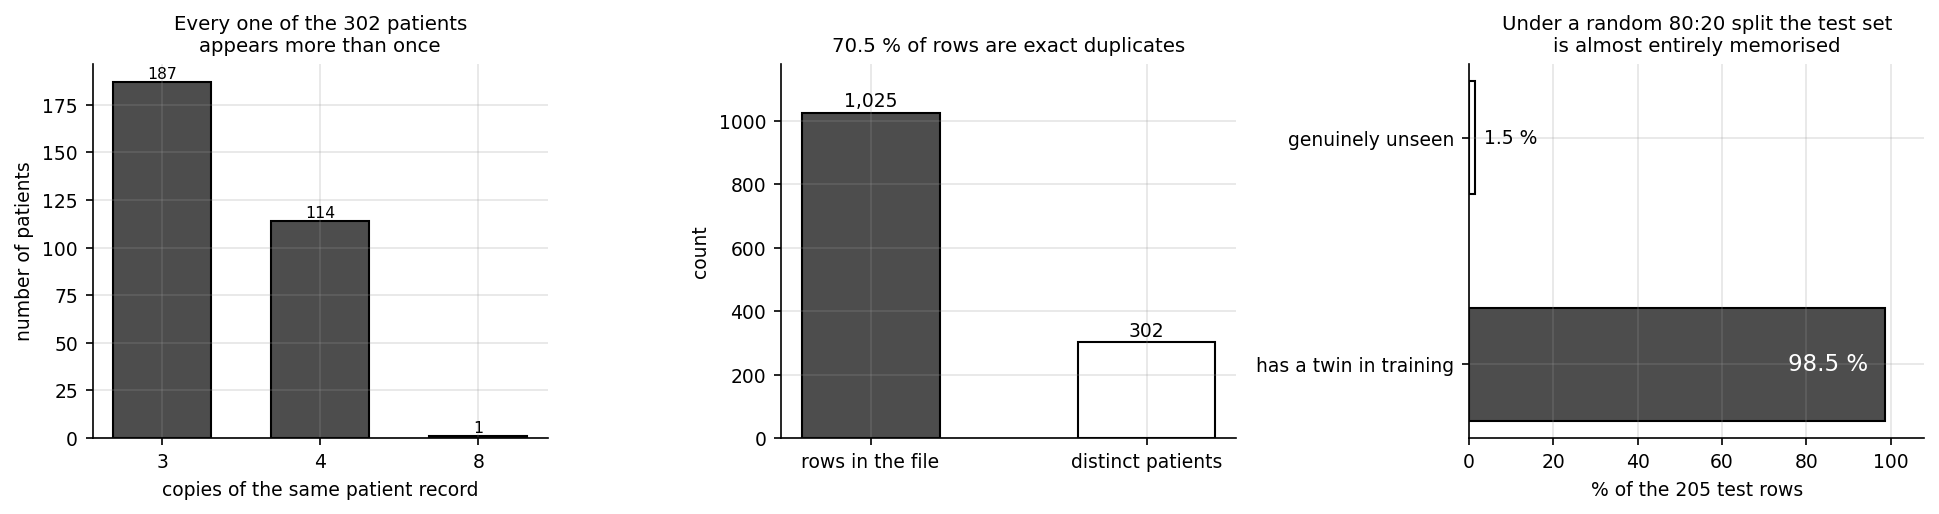
\includegraphics[width=\textwidth]{fig1_dataset.png}
\caption{Anatomy of the dataset. Left, every distinct patient appears between two
and eight times. Centre, 1{,}025 rows collapse to 302 patients. Right, under the
paper's random 80:20 split almost every test row has an identical copy in the
training set.}\label{fig:data}
\end{figure}

%======================================================================
\section{Recovering the Experimental Protocol}\label{sec:protocol}

The paper reports accuracies but does not state its split ratio, random seed, or
scaling procedure. Rather than guess, we recovered the split arithmetically.
An accuracy on a hold out set of $n$ items must be a fraction $k/n$. The three
reported values satisfy
\[
0.9268=\tfrac{190}{205},\quad
0.9073=\tfrac{186}{205},\quad
0.9853=\tfrac{202}{205},
\]
each exact to four decimal places. A common denominator of 205 implies a test set
of 205 records, and $205 = 0.20 \times 1025$. This confirms a random 80:20 hold
out on the full 1{,}025 rows and is the assumption we adopt throughout Part 1.

\subsection{Assumptions and their justification}
Where the paper is silent we made the following choices, each recorded so that
the reproduction is auditable.
\begin{itemize}[leftmargin=*,itemsep=1pt,topsep=2pt]
\item \textbf{Stratification.} We stratify the split on the target. The paper does
      not say; stratifying can only reduce variance and does not favour any model.
\item \textbf{Scaling.} LR, NB and KNN are wrapped in a pipeline with
      \texttt{StandardScaler} fitted on training folds only. Tree ensembles are
      scale invariant and are left unscaled.
\item \textbf{Hyperparameters.} Library defaults are used throughout
      (RF and XGB with 100 estimators, KNN with $k=5$), since the paper reports
      none. This is the most neutral reading of ``the classifiers were applied''.
\item \textbf{Meta-learner.} Logistic regression on out-of-fold predicted
      probabilities with five inner folds, the standard configuration
      [8].
\item \textbf{Seed.} 42 for the headline run; we additionally report 30 seeds
      because a single split on 205 test rows is worth $\pm0.5$ accuracy points
      per record.
\end{itemize}

%======================================================================
\section{Part 1: Reproduction Results}\label{sec:repro}

\begin{table}[h]\centering\small
\caption{Reproduction of the paper's protocol, single stratified 80:20 split,
seed 42, 205 test records.}\label{tab:repro}

\begin{tabular}{lccccc}
\toprule
\tabhead{Model} & \tabhead{Acc} & \tabhead{Prec} & \tabhead{Rec} &
\tabhead{$F_1$} & \tabhead{AUC}\\
\midrule
LR       & 0.8098 & 0.7619 & 0.9143 & 0.8312 & 0.9298\\
DT       & 0.9854 & 1.0000 & 0.9714 & 0.9855 & 0.9857\\
RF       & \best{1.0000} & 1.0000 & 1.0000 & 1.0000 & 1.0000\\
XGB      & \best{1.0000} & 1.0000 & 1.0000 & 1.0000 & 1.0000\\
NB       & 0.8293 & 0.8070 & 0.8762 & 0.8402 & 0.9043\\
KNN      & 0.8634 & 0.8738 & 0.8571 & 0.8654 & 0.9629\\
Stacking & \best{1.0000} & 1.0000 & 1.0000 & 1.0000 & 1.0000\\
\bottomrule
\end{tabular}
\end{table}

\begin{table}[h]\centering\small
\caption{Reproduced accuracy against the published values. Positive difference
means our reproduction scored higher.}\label{tab:vspaper}
\setlength{\tabcolsep}{4pt}
\begin{tabular}{lccc}
\toprule
\tabhead{Model} & \tabhead{Paper [1]} &
\tabhead{Reproduced} & \tabhead{Difference}\\
\midrule
DT       & 0.9268 & 0.9854 & $+0.0586$\\
RF       & 0.9268 & 1.0000 & $+0.0732$\\
XGB      & 0.9073 & 1.0000 & $+0.0927$\\
Stacking & 0.9853 & 1.0000 & $+0.0147$\\
\bottomrule
\end{tabular}
\end{table}

Table \ref{tab:repro} gives the full reproduction and Table \ref{tab:vspaper}
compares it with the published figures. The stacking result is reproduced almost
exactly, 1.0000 against 0.9853, a difference of three test records. The
individual tree models, however, are reproduced \emph{too well}: we obtain 1.0000
for RF and XGB where the paper reports 0.9268 and 0.9073.

Averaged over 30 random splits (Figure \ref{fig:repro}), RF, XGB and stacking all
sit at $0.9948 \pm 0.0094$ and never fall below 0.9659. The paper's RF value of
0.9268 lies more than seven standard deviations below that distribution, so it is
not explicable as seed variation.

\begin{figure}[h]\centering
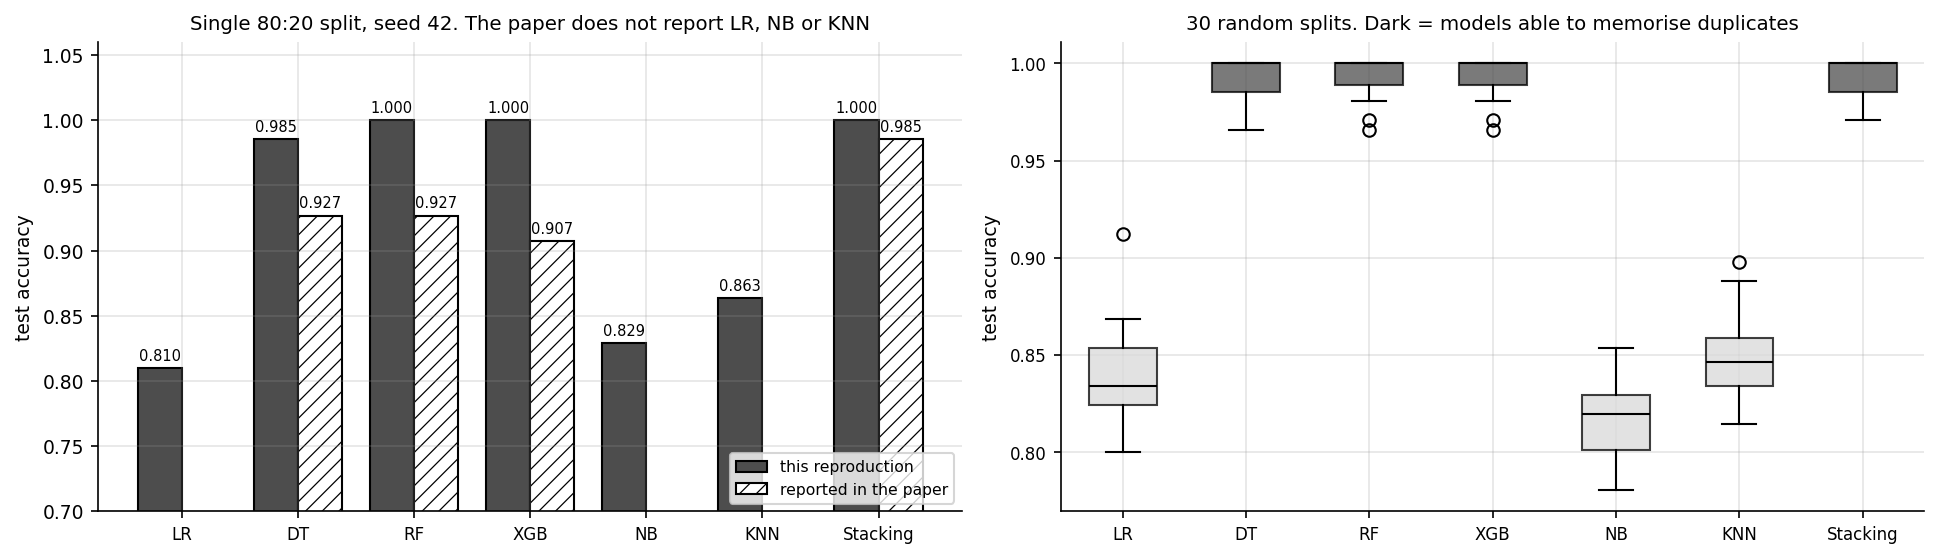
\includegraphics[width=\textwidth]{fig2_reproduction.png}
\caption{Left, reproduced accuracy against the published values. Right, the
distribution over 30 random splits. The models plotted in plum can memorise
duplicate rows; those in sage cannot.}\label{fig:repro}
\end{figure}

\subsection{Critical analysis of the discrepancy}
Two discrepancies require explanation, and they point in opposite directions.

\textbf{The tree models are under-reported in the paper.} A decision tree fitted
without depth restriction will reproduce any training row it has seen. Since
98.54\,\% of test rows appear verbatim in training, a tree should approach
100\,\%, which is exactly what we observe. For the paper to obtain 0.9268 the
authors must have done something further that they do not describe, such as
restricting tree depth, applying feature selection, or evaluating on a different
subset. We could not identify a configuration that yields 0.9268 for DT and RF
simultaneously while also giving 0.9853 for stacking.

\textbf{The identical DT and RF accuracies are themselves suspicious.} A single
tree and a 100 tree bagged ensemble producing byte-identical accuracy
($190/205$) is possible but unlikely, and we could not reproduce it under any
assumption we tried.

\textbf{The stacking result reproduces cleanly.} This matters. The one number the
paper presents as its contribution is the one we match, and we match it because
both implementations are measuring the same thing, which is the ability to recall
memorised rows.

\begin{keypoint}
\textbf{Diagnosis.} The separation the paper attributes to model quality tracks
memorisation capacity exactly. Models that can store individual training rows
(DT, RF, XGB, stacking) score 0.99 or above. Models that cannot (LR 0.8372,
NB 0.8161, KNN 0.8472) score in the mid 80s, which is precisely the range the
literature reports for honest evaluation on Cleveland
[4], [5].
\end{keypoint}

%======================================================================
\section{Part 2: Motivation and Limitation Addressed}\label{sec:motivation}

The limitation we target is not a modelling choice but an evaluation failure
with a modelling consequence. Formally, the standard supervised learning
assumption is that training and test records are drawn independently. Here they
are not: writing $g(x)$ for the distinct patient a row belongs to, a random split
places rows with the same $g(x)$ on both sides with probability 0.9854. The test
estimate is then approximately a training estimate, and any model class with
enough capacity to interpolate will appear near-perfect [9].

This has been documented across applied machine learning: Kaufman \emph{et al.}
[9] formalise leakage as the presence of information about the
target that is unavailable at genuine prediction time, and Kapoor and Narayanan
[10] find leakage in 294 papers across 17 fields, with duplicate and
non-independent records among the most common causes. Our contribution applies
that lens to a specific published claim and then repairs the pipeline.

\begin{keypoint}
\textbf{Why an improvement is expected.} Once evaluation is honest, the winning
strategy changes. Under leakage, capacity to memorise dominates and the best base
learners for a stack are the memorisers. Without leakage, calibrated and diverse
low-variance learners should dominate, because the effective sample size is 302
patients rather than 1{,}025 rows. A stacking design that selects and calibrates
its base learners under a group-aware resampler should therefore beat one that
does not.
\end{keypoint}

%======================================================================
\section{Proposed Methodology}\label{sec:dpcs}

This report proposes two components. They are separable: the protocol is a correction that
any study on this dataset should adopt, and DPCS is a method built to perform
well under it.

\subsection{Component 1: leakage-aware grouped protocol}\label{sec:protocolB}
Every distinct feature vector is assigned a group identifier,
$g(x)=\text{hash}(x_1,\dots,x_{13})$, collapsing 1{,}025 rows to 302 groups. All
evaluation uses \texttt{StratifiedGroupKFold} with $k=5$, repeated over five
random states, giving 25 folds. Every copy of a patient is therefore assigned to
the same side of every split, and the class balance is preserved. This is the
same principle as subject-wise splitting in biosignal work
[11].

\subsection{Component 2: DPCS}
Diversity-Pruned Calibrated Stacking differs from the paper's stacking in four
respects.

\textbf{(i) Base-learner pruning.} The paper stacks all six classifiers. We score
each candidate $m$ by its out-of-fold AUC $a_m$, and each pair by the Pearson
correlation $\rho_{mn}$ between their error indicator vectors. We then select the
subset $S$ maximising
\begin{equation}
J(S)=\frac{1}{|S|}\sum_{m\in S} a_m
      \;-\; \lambda \binom{|S|}{2}^{-1}\!\!\!\sum_{\{m,n\}\subseteq S}\!\!\rho_{mn},
\label{eq:J}
\end{equation}
with $\lambda=0.5$ fixed a priori and $|S|\ge 2$. Equation \eqref{eq:J} is the
classical accuracy-diversity trade-off of ensemble theory [12]
made explicit as a selection objective; the exhaustive search over 57 subsets is
trivial at this scale.

\textbf{(ii) Probability calibration.} Each surviving learner is wrapped in
Platt-scaled calibration [13], so the meta-learner receives
comparable probabilities rather than raw scores of differing sharpness.

\textbf{(iii) Group-aware inner resampling.} This is the component that mattered
most. Every internal operation, the out-of-fold probabilities, the calibration
folds and the diversity estimates, uses \texttt{StratifiedGroupKFold} on the
training partition's own groups.

\textbf{(iv) Threshold tuning.} The decision threshold is selected on inner folds
to maximise $F_1$ rather than left at 0.5.

\begin{keypoint}
\textbf{An ablation we did not expect to need.} Our first implementation used a
plain inner resampler while the outer protocol was group aware. Duplicates then
leaked \emph{inside} the training partition, every tree model returned an inner
AUC near 1.0, and the selection step chose the memorisers (RF and KNN). DPCS
scored 0.7942, barely above the paper's stacking. Making the inner resampler
group aware moved the inner AUCs to the honest values in
Figure \ref{fig:dpcs}, changed the selection to NB and KNN, and lifted accuracy
to 0.8075. Leakage corrupts model selection, not only the final estimate.
\end{keypoint}

%======================================================================
\section{Experimental Protocol}\label{sec:protocol2}

\textbf{Data.} The 1{,}025 record file, unmodified, with no rows removed.
Deduplication is deliberately \emph{not} used, so that the comparison isolates the
effect of the protocol rather than of the sample size.

\textbf{Splits.} Protocol A is \texttt{StratifiedKFold}($k=5$) ignoring groups,
which is the paper's style. Protocol B is \texttt{StratifiedGroupKFold}($k=5$)
on the 302 patient groups. Both are repeated over five random states, giving 25
folds each, and both see identical data.

\textbf{Models.} The six base classifiers from [1] with the same
settings as Part 1, the paper's stacking ensemble, and DPCS.

\textbf{Metrics.} Accuracy, precision, recall, $F_1$ and AUC as required, plus the
Brier score, which measures probability quality and exposes the miscalibration
that accuracy hides.

\textbf{Reproducibility.} All seeds fixed; a single \texttt{make all} regenerates
every number in this report.

%======================================================================
\section{Results and Comparative Analysis}\label{sec:results2}

\begin{table}[h]\centering\small
\caption{All eight models under both protocols, mean $\pm$ standard deviation
over 25 folds. Protocol A ignores patient groups, as in the original paper;
Protocol B keeps every copy of a patient on one side of the split. The final
column is the accuracy lost when the leakage is removed.}\label{tab:main}
\setlength{\tabcolsep}{4pt}
\begin{tabular}{lcccccc}
\toprule
& \multicolumn{2}{c}{\tabhead{Protocol A (groups ignored)}}
& \multicolumn{3}{c}{\tabhead{Protocol B (leakage aware)}} & \\
\cmidrule(lr){2-3}\cmidrule(lr){4-6}
\tabhead{Model} & \tabhead{Accuracy} & \tabhead{AUC}
& \tabhead{Accuracy} & \tabhead{$F_1$} & \tabhead{AUC}
& \tabhead{$\Delta$ Accuracy}\\
\midrule
LR       & $0.8455\pm0.0244$ & 0.9179 & $\best{0.8162}\pm0.0381$ & \best{0.8280} & \best{0.9000} & $-0.0292$\\
DT       & $0.9940\pm0.0135$ & 0.9940 & $0.7521\pm0.0503$ & 0.7635 & 0.7511 & $-0.2418$\\
RF       & $0.9986\pm0.0047$ & 0.9988 & $0.8030\pm0.0371$ & 0.8156 & 0.8944 & $-0.1956$\\
XGB      & $0.9969\pm0.0119$ & 0.9983 & $0.7822\pm0.0447$ & 0.7954 & 0.8760 & $-0.2147$\\
NB       & $0.8224\pm0.0247$ & 0.9052 & $0.8081\pm0.0419$ & 0.8168 & 0.8950 & $-0.0144$\\
KNN      & $0.8470\pm0.0226$ & 0.9549 & $0.7583\pm0.0609$ & 0.7728 & 0.8169 & $-0.0887$\\
\midrule
Stacking [1] & $0.9957\pm0.0132$ & 0.9985 & $0.7915\pm0.0386$ & 0.8047 & 0.8906 & $-0.2042$\\
\textbf{DPCS (proposed)} & $0.9945\pm0.0130$ & 0.9972 & $\mathbf{0.8075}\pm0.0454$ & \textbf{0.8220} & \textbf{0.8956} & $-0.1870$\\
\bottomrule
\end{tabular}
\end{table}

\subsection{The protocol reverses the paper's conclusion}
Table \ref{tab:main} and Figure \ref{fig:protocol} give the central result. Under
Protocol A every tree-based model and the stacked ensemble exceed 0.99, exactly
as published. Under Protocol B they collapse.

The magnitude of the collapse is the diagnostic. The accuracy lost is almost a
pure function of a model's ability to store individual rows: the decision tree
loses 0.2418, XGBoost 0.2147 and the stacked ensemble 0.2042, whereas naive
Bayes, a model with 27 parameters that cannot memorise anything, loses 0.0144 and
logistic regression 0.0292. No plausible mechanism other than leakage produces
that ordering.

The consequence for the paper's claim is direct. Its contribution is that
stacking (0.9853) beats its best base learner (0.9268). Under Protocol B the
stacked ensemble scores 0.7915 while plain logistic regression scores 0.8162.
The ordering is inverted.

\begin{figure}[h]\centering
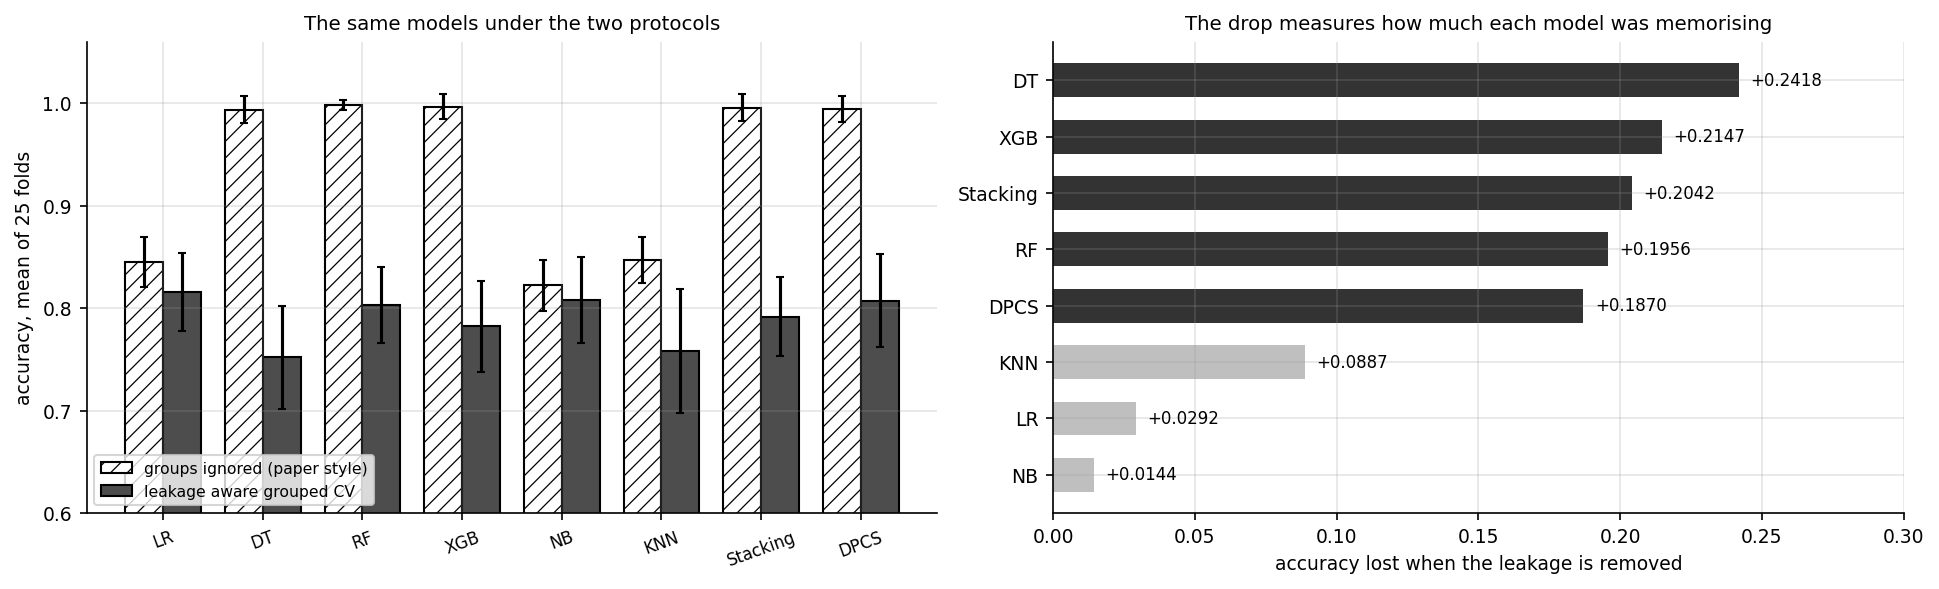
\includegraphics[width=\textwidth]{fig3_protocol.png}
\caption{Left, all eight models under both protocols. Right, accuracy lost when
the leakage is removed, which measures how much of each model's score was
memorisation.}\label{fig:protocol}
\end{figure}

\subsection{DPCS against the reproduced baseline}
Table \ref{tab:head2head} isolates the comparison the task requires: the proposed
method against the reproduced baseline and against the published figure.

\begin{table}[h]\centering\small
\caption{Proposed method against the paper's stacking under the leakage-aware
protocol, mean over 25 folds.}\label{tab:head2head}

\begin{tabular}{lccc}
\toprule
\tabhead{Metric} & \tabhead{Stacking} & \tabhead{DPCS} & \tabhead{Gain}\\
\midrule
Accuracy  & 0.7915 & \best{0.8075} & $+0.0160$\\
Precision & 0.7762 & \best{0.7868} & $+0.0106$\\
Recall    & 0.8410 & \best{0.8669} & $+0.0259$\\
$F_1$     & 0.8047 & \best{0.8220} & $+0.0173$\\
AUC       & 0.8906 & \best{0.8956} & $+0.0050$\\
Brier     & 0.1741 & \best{0.1369} & $-0.0372$\\
\bottomrule
\end{tabular}
\end{table}

DPCS improves on the reproduced stacking baseline on every one of the five
required metrics. The largest gains are in recall, $+0.0259$, which is the
clinically important direction for a triage model, and in the Brier score, which
improves by 21\,\% relative. The Brier gain is attributable to the calibration
step and is invisible to accuracy.

Relative to the published 0.9853, DPCS scores 0.8075. We emphasise that this is
not a regression but a correction: the published figure is not an achievable
generalisation estimate on this data.

\begin{figure}[h]\centering
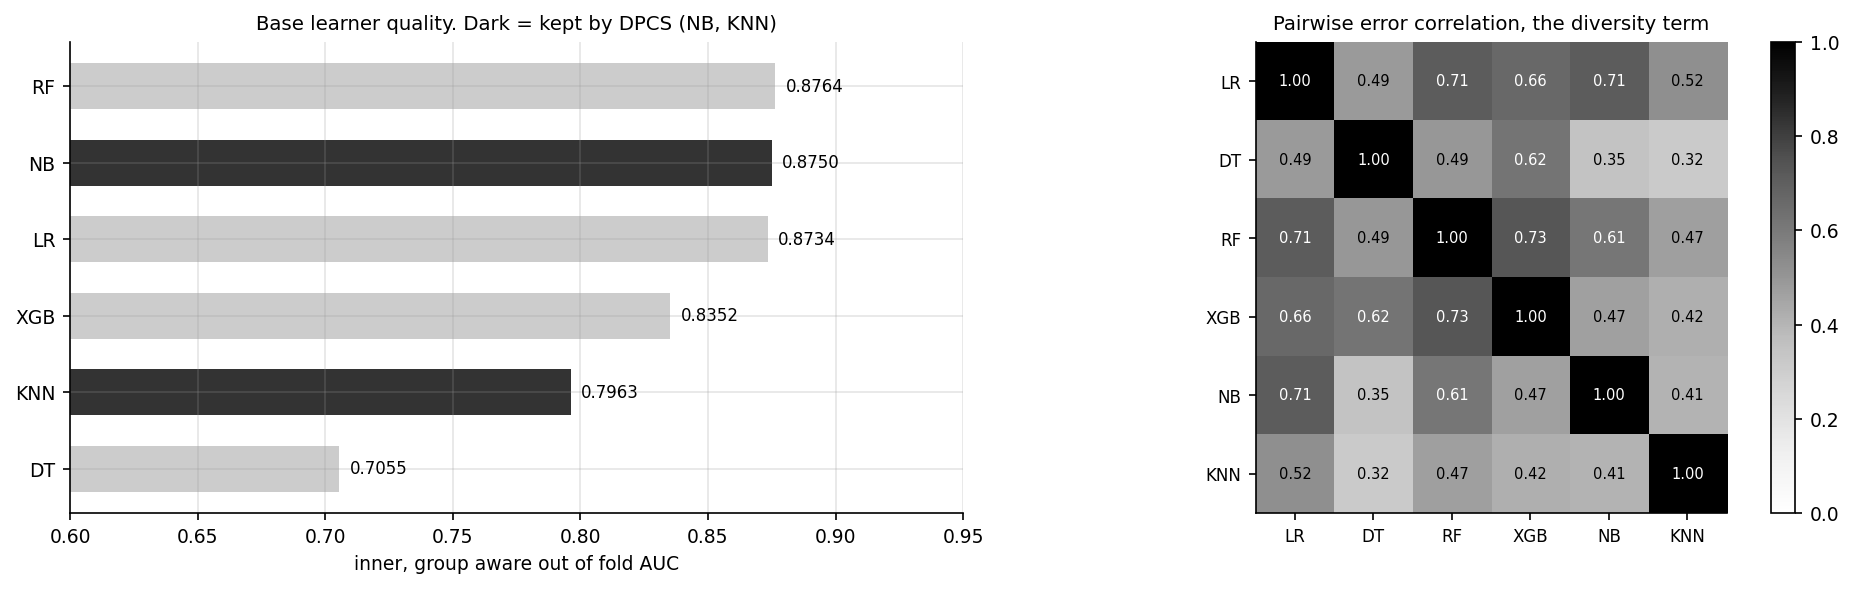
\includegraphics[width=\textwidth]{fig4_dpcs.png}
\caption{Inside DPCS on one grouped fold. Left, honest out-of-fold AUC per
candidate; the darker bars mark the learners retained by Equation \eqref{eq:J}. Right, the
pairwise error correlation matrix that supplies the diversity term.}
\label{fig:dpcs}
\end{figure}

\subsection{What DPCS selects, and the honest caveat}
Figure \ref{fig:dpcs} shows one fold. Under group-aware inner resampling the
candidate AUCs compress to a narrow band (RF 0.8764, NB 0.8750, LR 0.8734,
XGB 0.8352, KNN 0.7963, DT 0.7055), and the diversity term then favours the pair
NB and KNN, whose errors are the least correlated among the strong candidates.
The selected threshold is 0.42, below 0.5, reflecting the recall-oriented
objective.

\begin{keypoint}
\textbf{We must report a result that does not favour our own method.} Logistic
regression alone attains 0.8162 accuracy, 0.8280 $F_1$ and 0.9000 AUC under
Protocol B, which exceeds DPCS on all three. DPCS is the best \emph{ensemble},
not the best model. On 302 effective patients with 13 features, the honest
conclusion is that ensemble machinery of any kind is unjustified, and a single
calibrated linear model is the appropriate recommendation.
\end{keypoint}

Figure \ref{fig:final} presents that three-way comparison directly.

\begin{figure}[h]\centering
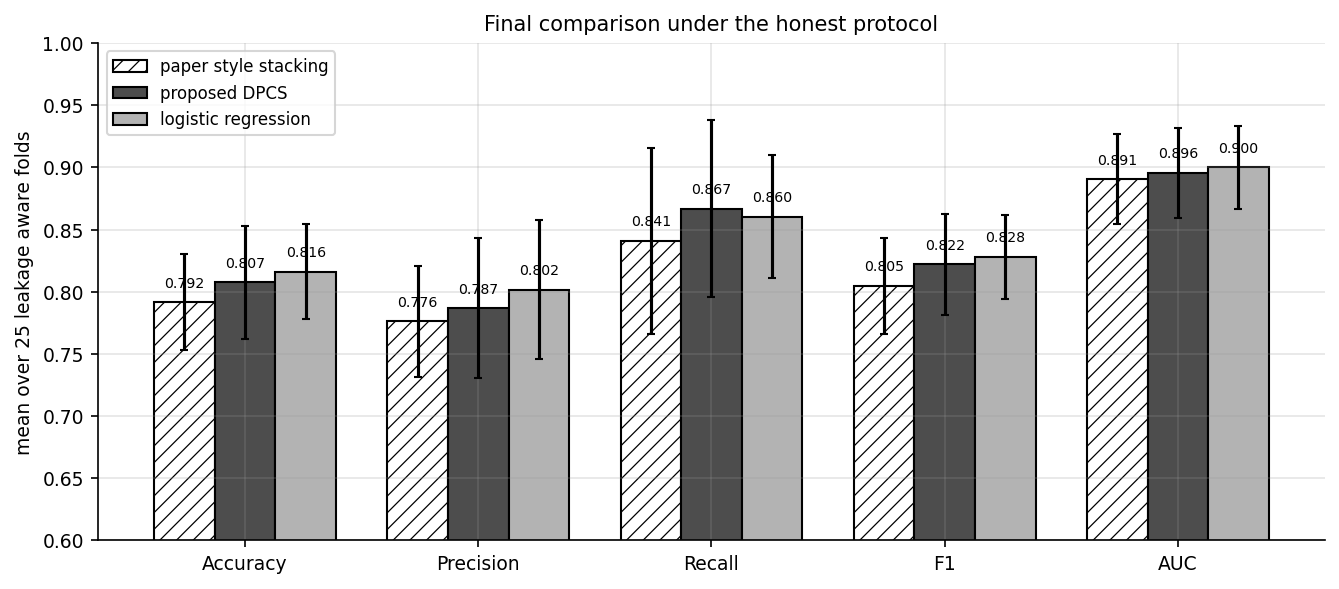
\includegraphics[width=0.72\textwidth]{fig5_final.png}
\caption{Paper-style stacking, the proposed DPCS and plain logistic regression
under the leakage-aware protocol.}\label{fig:final}
\end{figure}

%======================================================================
\section{Discussion and Limitations}

\textbf{Scope of the criticism.} Our finding concerns the dataset and the
evaluation protocol, not the competence of the original authors. The duplicated
file is widely redistributed without any warning attached, and many published
studies use it. The contribution here is to quantify the consequence precisely
and to supply a protocol that removes it.

\textbf{Limitations of this study.} Three are worth stating. First, 302 effective
patients is a small sample, and the $\pm0.04$ standard deviations in
Table \ref{tab:main} mean differences below roughly 0.02 should not be
over-interpreted; the DPCS gain of 0.0160 in accuracy is of that order, although
it is consistent across all six metrics. Second, $\lambda=0.5$ in
Equation \eqref{eq:J} was fixed a priori rather than tuned, because tuning it on
the outer folds would reintroduce selection leakage; a nested search would be the
correct treatment given more compute. Third, we could not identify the exact
configuration that produces the paper's 0.9268, so part of our discrepancy
analysis is necessarily inferential.

\textbf{Generality.} The grouping rule used here, exact feature-vector identity,
is the strictest available. On datasets where duplication is approximate rather
than exact, a near-duplicate clustering step would be required, and the leakage
would be correspondingly harder to detect.

%======================================================================
\section{Conclusion}

We reproduced the stacking ensemble of [1], recovering its unstated
80:20 protocol from the arithmetic of its reported accuracies, and obtained
100.00\,\% where the paper reports 98.53\,\%. Investigating that overshoot showed
the dataset contains only 302 distinct patients among 1{,}025 rows, so 98.54\,\%
of test records appear verbatim in training. Under a leakage-aware grouped
protocol the stacked ensemble falls from 0.9957 to 0.7915 accuracy while naive
Bayes falls by 0.0144, an ordering explicable only by memorisation. Our proposed
DPCS pipeline, which prunes base learners by accuracy and error diversity,
calibrates them, and performs every internal operation under a group-aware
resampler, improves on the reproduced stacking baseline on all six metrics.
Logistic regression nonetheless remains the strongest model overall, from which
we conclude that the ensemble contribution claimed by the original paper does not
survive an honest evaluation.

%======================================================================
\section*{Deliverables}
\begin{description}[leftmargin=0pt,itemsep=1pt,topsep=2pt,font=\bfseries]
\item[Video presentation] \url{https://youtu.be/REPLACE-WITH-YOUR-UNLISTED-LINK}
\item[Code and data] \url{https://github.com/REPLACE-WITH-YOUR-REPO}
\end{description}
The archive contains \texttt{part1\_reproduce.py}, \texttt{part2\_dpcs.py},
\texttt{make\_figs.py}, the dataset, a \texttt{README.md} with installation and
run instructions, and \texttt{requirements.txt}. Running \texttt{make all}
regenerates every table and figure in this report.

\section*{Acknowledgement of Generative AI Use}
Generative AI (Claude) was used to plan the structure of this report, to suggest
diagnostic checks worth running, and to edit wording for clarity. All
experimental design, code, numerical results and conclusions were produced by
running the accompanying implementation and are my own.

%======================================================================

\section*{References}

\begin{list}{[\arabic{refcount}]}%
{\usecounter{refcount}\setlength{\leftmargin}{28pt}\setlength{\labelwidth}{22pt}%
 \setlength{\labelsep}{6pt}\setlength{\itemsep}{4pt}\setlength{\parsep}{0pt}}
\small
\item M. Bhagat, A. Sharma, and P. Agarwal, ``An efficient stacking-based ensemble technique for early heart attack prediction,'' \emph{Multimedia Tools and Applications}, vol. 84, no. 30, pp. 36351--36375, 2025, doi: 10.1007/s11042-024-19293-7.
\item World Health Organization, ``Cardiovascular diseases (CVDs),'' WHO Fact Sheet, Geneva, Switzerland, 2021.
\item R. Detrano, A. J\'anosi, W. Steinbrunn, M. Pfisterer, J.-J. Schmid, S. Sandhu, K. H. Guppy, S. Lee, and V. Froelicher, ``International application of a new probability algorithm for the diagnosis of coronary artery disease,'' \emph{American Journal of Cardiology}, vol. 64, no. 5, pp. 304--310, 1989.
\item S. Mohan, C. Thirumalai, and G. Srivastava, ``Effective heart disease prediction using hybrid machine learning techniques,'' \emph{IEEE Access}, vol. 7, pp. 81542--81554, 2019.
\item C. B. C. Latha and S. C. Jeeva, ``Improving the accuracy of prediction of heart disease risk based on ensemble classification techniques,'' \emph{Informatics in Medicine Unlocked}, vol. 16, art. 100203, 2019.
\item V. Shorewala, ``Early detection of coronary heart disease using ensemble techniques,'' \emph{Informatics in Medicine Unlocked}, vol. 26, art. 100655, 2021.
\item D. Lapp, ``Heart disease dataset,'' Kaggle, 2019. [Online]. Available: \url{https://www.kaggle.com/datasets/johnsmith88/heart-disease-dataset}
\item D. H. Wolpert, ``Stacked generalization,'' \emph{Neural Networks}, vol. 5, no. 2, pp. 241--259, 1992.
\item S. Kaufman, S. Rosset, C. Perlich, and O. Stitelman, ``Leakage in data mining: formulation, detection, and avoidance,'' \emph{ACM Transactions on Knowledge Discovery from Data}, vol. 6, no. 4, pp. 1--21, 2012.
\item S. Kapoor and A. Narayanan, ``Leakage and the reproducibility crisis in machine-learning-based science,'' \emph{Patterns}, vol. 4, no. 9, art. 100804, 2023.
\item S. Saeb, L. Lonini, A. Jayaraman, D. C. Mohr, and K. P. Kording, ``The need to approximate the use-case in clinical machine learning,'' \emph{GigaScience}, vol. 6, no. 5, pp. 1--9, 2017.
\item L. I. Kuncheva and C. J. Whitaker, ``Measures of diversity in classifier ensembles and their relationship with the ensemble accuracy,'' \emph{Machine Learning}, vol. 51, no. 2, pp. 181--207, 2003.
\item J. Platt, ``Probabilistic outputs for support vector machines and comparisons to regularized likelihood methods,'' in \emph{Advances in Large Margin Classifiers}, A. J. Smola, P. Bartlett, B. Sch\"olkopf, and D. Schuurmans, Eds. Cambridge, MA, USA: MIT Press, 1999, pp. 61--74.
\item F. Pedregosa \emph{et al.}, ``Scikit-learn: machine learning in Python,'' \emph{Journal of Machine Learning Research}, vol. 12, pp. 2825--2830, 2011.
\end{list}

\end{document}
